%!TEX program = xelatex

\documentclass[a4paper, openany, oneside]{memoir}
\usepackage[no-math]{fontspec}
\usepackage{pgfplots}
\pgfplotsset{compat=newest}
\usepackage{commath}
\usepackage{mathtools}
\usepackage{amssymb}
\usepackage{amsthm}
\usepackage{booktabs}
\usepackage{mathtools}
\usepackage{xcolor}
\usepackage[separate-uncertainty=true, per-mode=symbol]{siunitx}
\usepackage[noabbrev, capitalize]{cleveref}
\usepackage{listings}
\usepackage[american inductor, european resistor]{circuitikz}
\usepackage{amsmath}
\usepackage{amsfonts}
\usepackage{ifxetex}
\usepackage[dutch,english]{babel}
\usepackage[backend=bibtexu,texencoding=utf8,bibencoding=utf8,style=ieee,sortlocale=en_GB,language=auto]{biblatex}
\usepackage[strict,autostyle]{csquotes}
\usepackage{parskip}
\usepackage{import}
\usepackage{standalone}
\usepackage{hyperref}
%\usepackage[toc,title,titletoc]{appendix}

\ifxetex{} % Fonts laden in het geval dat je met Xetex compiled
    \usepackage{fontspec}
    \defaultfontfeatures{Ligatures=TeX} % To support LaTeX quoting style
    \setromanfont{Palatino Linotype} % Tover ergens in Font mapje in root.
    \setmonofont{Source Code Pro}
\else % Terug val in standaard pdflatex tool chain. Geen ondersteuning voor OTT fonts
    \usepackage[T1]{fontenc}
    \usepackage[utf8]{inputenc}
\fi
\newcommand{\references}[1]{\begin{flushright}{#1}\end{flushright}}
\renewcommand{\vec}[1]{\boldsymbol{\mathbf{#1}}}
\newcommand{\uvec}[1]{\boldsymbol{\hat{\vec{#1}}}}
\newcommand{\mat}[1]{\boldsymbol{\mathbf{#1}}}
\newcommand{\fasor}[1]{\boldsymbol{\tilde{\vec{#1}}}}
\newcommand{\cmplx}[0]{\mathrm{j}}
\renewcommand{\Re}[0]{\operatorname{Re}}
\newcommand{\Cov}{\operatorname{Cov}}
\newcommand{\Var}{\operatorname{Var}}
\newcommand{\proj}{\operatorname{proj}}
\newcommand{\Perp}{\operatorname{perp}}
\newcommand{\col}{\operatorname{col}}
\newcommand{\rect}{\operatorname{rect}}
\newcommand{\sinc}{\operatorname{sinc}}
\newcommand{\IT}{\operatorname{IT}}
\newcommand{\F}{\mathcal{F}}

\newtheorem{definition}{Definition}
\newtheorem{theorem}{Theorem}


\DeclareSIUnit{\voltampere}{VA} %apparent power
\DeclareSIUnit{\pii}{\ensuremath{\pi}}

\hypersetup{%setup hyperlinks
    colorlinks,
    citecolor=black,
    filecolor=black,
    linkcolor=black,
    urlcolor=black
}

% Example boxes
\usepackage{fancybox}
\usepackage{framed}
\usepackage{adjustbox}
\newenvironment{simpages}%
{\AtBeginEnvironment{itemize}{\parskip=0pt\parsep=0pt\partopsep=0pt}
\def\FrameCommand{\fboxsep=.5\FrameSep\shadowbox}\MakeFramed{\FrameRestore}}%
{\endMakeFramed}

% Impulse train
\DeclareFontFamily{U}{wncy}{}
\DeclareFontShape{U}{wncy}{m}{n}{<->wncyr10}{}
\DeclareSymbolFont{mcy}{U}{wncy}{m}{n}
\DeclareMathSymbol{\Sha}{\mathord}{mcy}{"58}
\addbibresource{../../../../includes/bibliography.bib}

\begin{document}

\subsection{Collaborative sampling}
In collaborative sampling, the estimation of the lags is split across two physically separate devices. This situation is analysed and described more carefully in \cref{ap:circ-ruler}. The advantage of splitting the estimation of the lags across physically separate devices is that this reduces the workload of a single device. 

To ensure that reconstruction is possible, we consider a treatment similar to \cref{sub:ci-circ}. However, the difference is that Step 6 of the reconstruction algorithm is invalid, since a single device does not satisfy the circular sparse ruler problem. However, since the device does estimate certain lags, an analysis similar \cref{sec:reconstruction-derivation} shows that each device solves its own part of the equation of Step 6 in such a way that their results yield the complete solution. Therefore, after the reconstruction of each device, it remains to combine their results. A possible final implementation is pictured in \cref{tkz:sc_collaborative_combine}.

\begin{figure}
\centering
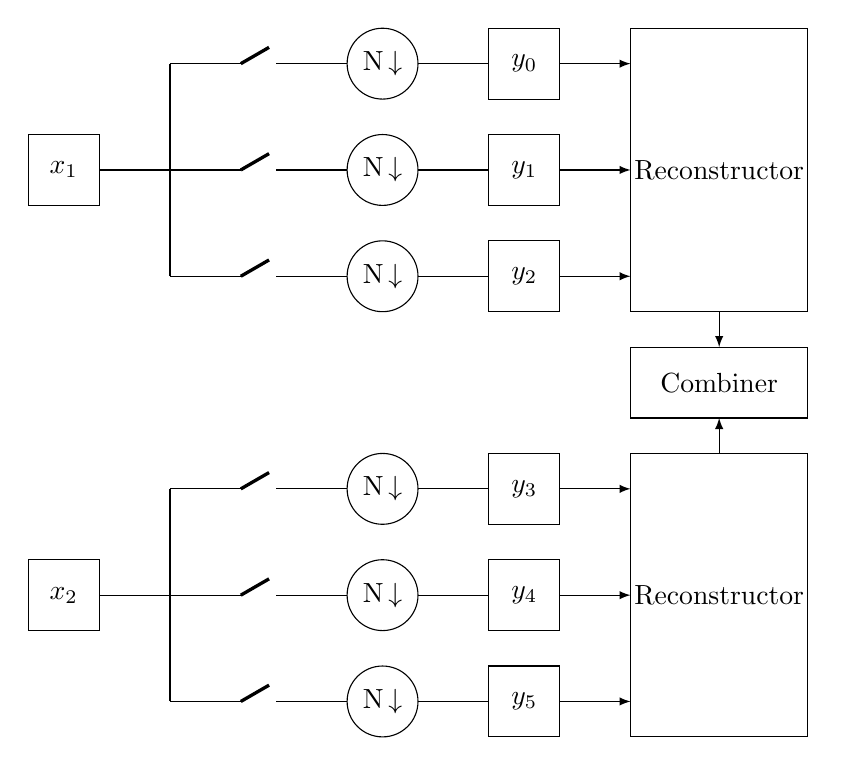
\begin{tikzpicture}[scale=.9]
\draw  (-2.5,2) rectangle (-1.5,1) node[pos=.5]{$x_1$};
\draw  (-1.5,1.5) -- (0.5,1.5);
\draw  (-0.5,3) -- (0.5,3);
\draw (-0.5,3) --(-.5,0) ;

\draw (-0.5,0) -- (0.5,0);

\draw  (1,3) -- (2,3);
\draw  (1,1.5) -- (2,1.5);
\draw  (1,0) -- (2,0);

\draw[ very thick](0.5,3)-- +(30:0.46);
\draw[ very thick](0.5,1.5)-- +(30:0.46);
\draw[ very thick](0.5,0)-- +(30:0.46);

\draw  (2.5,3) ellipse (.5 and .5) node{N$\,\downarrow$} ;
\draw  (2.5,1.5) ellipse (.5 and .5) node{N$\,\downarrow$} ;
\draw  (2.5,0) ellipse (.5 and .5) node{N$\,\downarrow$} ;

\draw  [>=latex,->] (5,3) -- (6,3);
\draw  [>=latex,->] (5,1.5) -- (6,1.5);
\draw  [>=latex,->] (5,0) -- (6,0);

\draw  (3,3) -- (4,3);
\draw  (3,1.5) -- (4,1.5);
\draw  (3,0) -- (4,0);

\draw  (5,3.5) rectangle (4,2.5) node[pos=.5]{$y_0$};
\draw  (5,2) rectangle (4,1) node[pos=.5]{$y_1$};
\draw  (5,0.5) rectangle (4,-0.5) node[pos=.5]{$y_2$};

\draw  (-2.5,-4) rectangle (-1.5,-5) node[pos=.5]{$x_2$};
\draw  (-1.5,-4.5) -- (0.5,-4.5);
\draw  (-0.5,-3) -- (0.5,-3);
\draw (-0.5,-3) --(-0.5,-6) ;

\draw (-0.5,-6) -- (0.5,-6);

\draw  (1,-3) -- (2,-3);
\draw  (1,-4.5) -- (2,-4.5);
\draw  (1,-6) -- (2,-6);

\draw[ very thick](0.5,-3)-- +(30:0.46);
\draw[ very thick](0.5,-4.5)-- +(30:0.46);
\draw[ very thick](0.5,-6)-- +(30:0.46);

\draw  (2.5,-3) ellipse (.5 and .5) node{N$\,\downarrow$} ;
\draw  (2.5,-4.5) ellipse (.5 and .5) node{N$\,\downarrow$} ;
\draw  (2.5,-6) ellipse (.5 and .5) node{N$\,\downarrow$} ;

\draw  (3,-3) -- (4,-3);
\draw  (3,-4.5) -- (4,-4.5);
\draw  (3,-6) -- (4,-6);

\draw  [>=latex,->] (5,-3) -- (6,-3);
\draw  [>=latex,->] (5,-4.5) -- (6,-4.5);
\draw  [>=latex,->] (5,-6) -- (6,-6);

\draw  (5,-2.5) rectangle (4,-3.5) node[pos=.5]{$y_3$};
\draw  (5,-4) rectangle (4,-5) node[pos=.5]{$y_4$};
\draw  (5,-5.5) rectangle (4,-6.5) node[pos=.5]{$y_5$};

\draw  (6,3.5) rectangle (8.5,-.5) node[pos=.5]{Reconstructor};
\draw  (6,-2.5) rectangle (8.5,-6.5) node[pos=.5]{Reconstructor};

\draw  (6,-1) rectangle (8.5,-2) node[pos=.5]{Combiner};
\draw [>=latex,->] (7.25,-2.5) -- (7.25,-2);
\draw [>=latex,->] (7.25,-.5) -- (7.25,-1);

\end{tikzpicture}
\caption{Schematic of collaborative sampling implementation with a combiner}\label{tkz:sc_collaborative_combine}
\end{figure}

% \subsection{combine collaborative sampler with reconstructor}\label{sub:ci-collab}
% To describe how every sampler behaves to the different reconstructors, we can use the same technique as described in \cref{sub:ci-circ}. We need different devices to compute different parts of the desired autocorrelation $\vec{r}_x$. Therefore we have to tell the reconstructor to not try to reconstruct the whole autocorrelation, but only parts of it per device. The results of different devices are then combined. However, it is not trivial to tell the reconstructor to only calculate the parts of the autocorrelation it has information for. do this we need to take a look at

% \begin{align} %\label{eq:ry-R-rx}
%     \vec{r}_y = \mat{R} \vec{r}_x.
% \end{align}
% which is the result from \cref{eq:ry-R-rx} in ref \todo{ref}. This formula describes the relationship between $\vec{r}_y$ and $\vec{r}_x$. When we don't have all lags available, $\mat{R}$ is not full column rank, what in practice means that there are columns with only zeros. These columns correspond directly to the elements of $\vec{r}_x$ we have no information of. So what we now need to do is remove the columns with only zeros, and remove the corresponding elements out of $\vec{r}_x$. One can choose to either calculate beforehand which columns are zero, but one can also do that after calculating $\mat{R}$, and remove the columns that are zero. 

% The only thing left to do is to combine the information on a combiner. This combiner takes the information of the different devices and puts their values accordingly in the autocorrelation vector $\vec{r}_x$. 


\end{document}
